% Options for packages loaded elsewhere
\PassOptionsToPackage{unicode}{hyperref}
\PassOptionsToPackage{hyphens}{url}
%
\documentclass[
  ignorenonframetext,
]{beamer}
\usepackage{pgfpages}
\setbeamertemplate{caption}[numbered]
\setbeamertemplate{caption label separator}{: }
\setbeamercolor{caption name}{fg=normal text.fg}
\beamertemplatenavigationsymbolsempty
% Prevent slide breaks in the middle of a paragraph
\widowpenalties 1 10000
\raggedbottom
\setbeamertemplate{part page}{
  \centering
  \begin{beamercolorbox}[sep=16pt,center]{part title}
    \usebeamerfont{part title}\insertpart\par
  \end{beamercolorbox}
}
\setbeamertemplate{section page}{
  \centering
  \begin{beamercolorbox}[sep=12pt,center]{part title}
    \usebeamerfont{section title}\insertsection\par
  \end{beamercolorbox}
}
\setbeamertemplate{subsection page}{
  \centering
  \begin{beamercolorbox}[sep=8pt,center]{part title}
    \usebeamerfont{subsection title}\insertsubsection\par
  \end{beamercolorbox}
}
\AtBeginPart{
  \frame{\partpage}
}
\AtBeginSection{
  \ifbibliography
  \else
    \frame{\sectionpage}
  \fi
}
\AtBeginSubsection{
  \frame{\subsectionpage}
}
\usepackage{lmodern}
\usepackage{amsmath}
\usepackage{ifxetex,ifluatex}
\ifnum 0\ifxetex 1\fi\ifluatex 1\fi=0 % if pdftex
  \usepackage[T1]{fontenc}
  \usepackage[utf8]{inputenc}
  \usepackage{textcomp} % provide euro and other symbols
  \usepackage{amssymb}
\else % if luatex or xetex
  \usepackage{unicode-math}
  \defaultfontfeatures{Scale=MatchLowercase}
  \defaultfontfeatures[\rmfamily]{Ligatures=TeX,Scale=1}
\fi
% Use upquote if available, for straight quotes in verbatim environments
\IfFileExists{upquote.sty}{\usepackage{upquote}}{}
\IfFileExists{microtype.sty}{% use microtype if available
  \usepackage[]{microtype}
  \UseMicrotypeSet[protrusion]{basicmath} % disable protrusion for tt fonts
}{}
\makeatletter
\@ifundefined{KOMAClassName}{% if non-KOMA class
  \IfFileExists{parskip.sty}{%
    \usepackage{parskip}
  }{% else
    \setlength{\parindent}{0pt}
    \setlength{\parskip}{6pt plus 2pt minus 1pt}}
}{% if KOMA class
  \KOMAoptions{parskip=half}}
\makeatother
\usepackage{xcolor}
\IfFileExists{xurl.sty}{\usepackage{xurl}}{} % add URL line breaks if available
\IfFileExists{bookmark.sty}{\usepackage{bookmark}}{\usepackage{hyperref}}
\hypersetup{
  pdftitle={Vector Autoregression},
  pdfauthor={Zahid Asghar},
  hidelinks,
  pdfcreator={LaTeX via pandoc}}
\urlstyle{same} % disable monospaced font for URLs
\newif\ifbibliography
\usepackage{graphicx}
\makeatletter
\def\maxwidth{\ifdim\Gin@nat@width>\linewidth\linewidth\else\Gin@nat@width\fi}
\def\maxheight{\ifdim\Gin@nat@height>\textheight\textheight\else\Gin@nat@height\fi}
\makeatother
% Scale images if necessary, so that they will not overflow the page
% margins by default, and it is still possible to overwrite the defaults
% using explicit options in \includegraphics[width, height, ...]{}
\setkeys{Gin}{width=\maxwidth,height=\maxheight,keepaspectratio}
% Set default figure placement to htbp
\makeatletter
\def\fps@figure{htbp}
\makeatother
\setlength{\emergencystretch}{3em} % prevent overfull lines
\providecommand{\tightlist}{%
  \setlength{\itemsep}{0pt}\setlength{\parskip}{0pt}}
\setcounter{secnumdepth}{-\maxdimen} % remove section numbering
\ifluatex
  \usepackage{selnolig}  % disable illegal ligatures
\fi

\title{Vector Autoregression}
\author{Zahid Asghar}
\date{5/19/2021}

\begin{document}
\frame{\titlepage}

\begin{frame}[fragile]{Vector Autoregressions (VARs)}
\protect\hypertarget{vector-autoregressions-vars}{}
\textbf{Primary Source: Stock, James H., and Mark W. Watson, ``Vector
Autoregressions,'' Journal of Economic Perspectives, Vol. 15 No.~4 (Fall
2001), 101-115.}

\emph{Macroeconometricians do 4 things}

\begin{verbatim}
1. Describe and summarize macroeconomic data, 

2. Make macroeconomic forecasts,  

3. Quantify what we know about the true structure of the macroeconomy, 

4. Advise or act as policymakers. 
\end{verbatim}

Following the problems of the 1970s, none of the structural models or
univariate time series approaches seemed trustworthy. VARs arose in this
vacuum.
\end{frame}

\begin{frame}[fragile]
\emph{VARs come in three varieties:}

\begin{verbatim}
 1. Reduced Form 

 2. Recursive 

 3. Structural 
\end{verbatim}

A \textbf{reduced-form} VAR expresses each variable as a linear function
of its own past values and the past values of all other variables being
considered and a serially uncorrelated error term.
\(\begin{aligned}\text{UNEM}_t = \beta_{10} &+ \beta_{11}\text{UNEM}_{t-1} + \beta_{12}\text{UNEM}_{t-2}\\&+ \gamma_{11}\text{INFL}_{t-1} + \gamma_{12}\text{INFL}_{t-2} \\&+ \phi_{11}\text{R}_{t-1} + \phi_{12}\text{R}_{t-2} \\&+ \mu_{1t}\end{aligned}\\ \ \\ \begin{aligned}\text{INFL}_t = \beta_{20} &+ \beta_{21}\text{UNEM}_{t-1} + \beta_{22}\text{UNEM}_{t-2}\\ &+ \gamma_{21}\text{INFL}_{t-1} + \gamma_{22}\text{INFL}_{t-2} \\&+ \phi_{21}\text{R}_{t-1} + \phi_{22}\text{R}_{t-2} \\&+ \mu_{2t}\end{aligned}\\ \ \\ \begin{aligned}\text{R}_t = \beta_{30} &+ \beta_{31}\text{UNEM}_{t-1} + \beta_{32}\text{UNEM}_{t-2}\\ &+ \gamma_{31}\text{INFL}_{t-1} + \gamma_{32}\text{INFL}_{t-2} \\&+ \phi_{31}\text{R}_{t-1} + \phi_{32}\text{R}_{t-2} \\&+ \mu_{3t}\end{aligned}\)

In theory, the VAR uses all available or relevant past values. In
practice, frequently the Akaike (AIC) or Bayes (BIC) information
criteria are used.

The error terms are viewed as ``surprises''---movements in the variables
after taking its past into account. If the different variables are
correlated with each other, then the error terms will also be correlated
across equations.
\end{frame}

\begin{frame}
A \textbf{recursive VAR} constructs the error terms in each regression
to be uncorrelated with the error term in the preceding equation. This
is done by adding carefully- selected contemporaneous values as
regressors. Estimation of each equation by OLS produces residuals that
are uncorrelated across equations.
\(\begin{aligned}\text{UNEM}_t = \beta_{10} &+ \beta_{11}\text{UNEM}_{t-1} + \beta_{12}\text{UNEM}_{t-2}\\&+ \gamma_{11}\text{INFL}_{t-1} + \gamma_{12}\text{INFL}_{t-2} \\&+ \phi_{11}\text{R}_{t-1} + \phi_{12}\text{R}_{t-2} \\&+ \mu_{1t}\end{aligned}\\ \ \\ \begin{aligned}\text{INFL}_t = \beta_{20} &+ \delta_{21}\text{UNEM}_{t} + \beta_{21}\text{UNEM}_{t-1} + \beta_{22}\text{UNEM}_{t-2}\\ &+ \gamma_{21}\text{INFL}_{t-1} + \gamma_{22}\text{INFL}_{t-2} \\&+ \phi_{21}\text{R}_{t-1} + \phi_{22}\text{R}_{t-2} \\&+ \mu_{2t}\end{aligned}\\ \ \\ \begin{aligned}\text{R}_t = \beta_{30} &+ \delta_{21}\text{UNEM}_{t} + \beta_{31}\text{UNEM}_{t-1} + \beta_{32}\text{UNEM}_{t-2}\\ &+ \delta_{31}\text{INFL}_{t} +\gamma_{31}\text{INFL}_{t-1} + \gamma_{32}\text{INFL}_{t-2} \\&+ \phi_{31}\text{R}_{t-1} + \phi_{32}\text{R}_{t-2} \\&+ \mu_{3t}\end{aligned}\)

The recursive VAR amounts to estimating the reduced form, then computing
the Cholesky factorization of the reduced form VAR covariance matrix.
(See the book by Lutkepohl, 1993).

Unfortunately the results depend on the order of the variables. Changing
the order changes the VAR equations, coefficients, and residuals, and
there are n! recursive VARs possible considering the possible
reorderings.

A \textbf{structural VAR} uses economic theory to sort out
contemporaneous links among the variables. Structural VARs require
``identifying assumptions'' that establish causal links among variables.
These produce instrumental variables.
\end{frame}

\begin{frame}[fragile]
Stock and Watson offer this example of a structural VAR based on a
Taylor rule:
\(R_t= r^*+1.5({\overline \pi_t - \pi^*})+1.25({\overline u_t - u^*})\)+
lagged values of \(R_t\),\(\pi_t\),\emph{u}+\(\epsilon_t\)

The asterisked values are desired values and bar values are 4 quarter
trailing averages. This equation becomes the interest rate equation in
the structural VAR.

\begin{verbatim}
 First the reduced form VAR and a recursive VAR are estimated to summarize the co-movements of the three series involved. 

Second, the reduced form VAR is used to forecast the variables. 

Third, the structural VAR is used to estimate the effect of a policy-induced change in the fed funds rate on inflation and unemployment. 
\end{verbatim}

\textbf{Standard practice} is to report

\begin{verbatim}
Granger-causality tests

impulse responses, and 

forecast error variance decompositions. 
\end{verbatim}

(These are more informative to understanding the relationships than the
VAR regression coefficients or \(R^2\) statistics.)
\end{frame}

\begin{frame}{Granger Causality}
\protect\hypertarget{granger-causality}{}
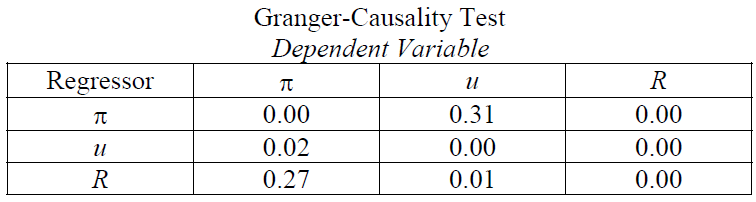
\includegraphics{/R_git/granger.png}

These are p-values for F-statistics for joint tests on lags. So
unemployment helps predict inflation (2\% level), but fed funds does not
help predict inflation (27\% level).

Here is a variance decomposition for the recursive VAR orders as π, u,
R. (1960-2000, quarterly). The variance decomposition (forecast error
decomposition) is the percentage of the variance of the error made in
forecasting a variable due to a specific shock at a specific time
horizon.
\end{frame}

\begin{frame}{Forecast Variance Error Deceomposition}
\protect\hypertarget{forecast-variance-error-deceomposition}{}
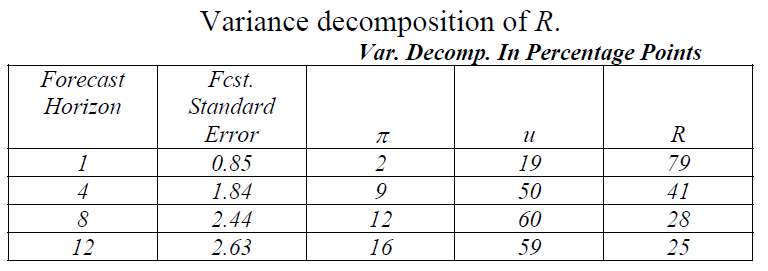
\includegraphics{/R_git/vardecomp.png} This suggests that 75\% of the
error in the forecast of the fed funds rate 12 quarters out is due to
inflation and unemployment shocks in the recursive VAR.

4Impulse responses trace out the response of current and future values
of each of the variables to a one-unit increase in the current value of
one of the VAR errors. It is a one period shock which reverts to zero
immediately. These make more sense in the context of a model with
uncorrelated errors across equations.
\end{frame}

\begin{frame}{Impulse Response Function}
\protect\hypertarget{impulse-response-function}{}
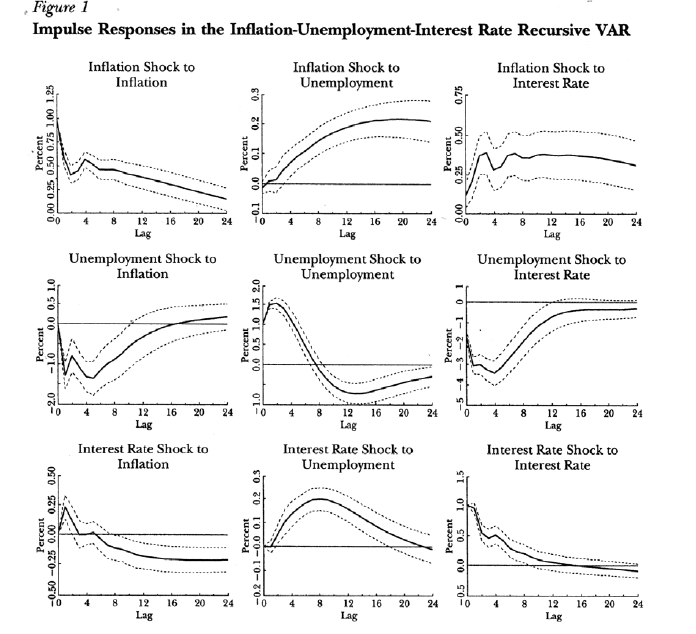
\includegraphics{/R_git/irf.png}

In these we see the effect of a 1\% change in each variable as it works
through the recursive VAR system with the coefficients estimated from
actual data. Also plotted are ±1 standard deviation error bands,
yielding roughly 66\% confidence intervals.

The reduced-form VAR model can also be used to iterate forward to
forecast. Stock and Watson then replace the interest rate equation with
two forms of the Taylor rule (one backward looking and one forward
looking), and compare impulse responses of monetary policy shocks.
\end{frame}

\begin{frame}
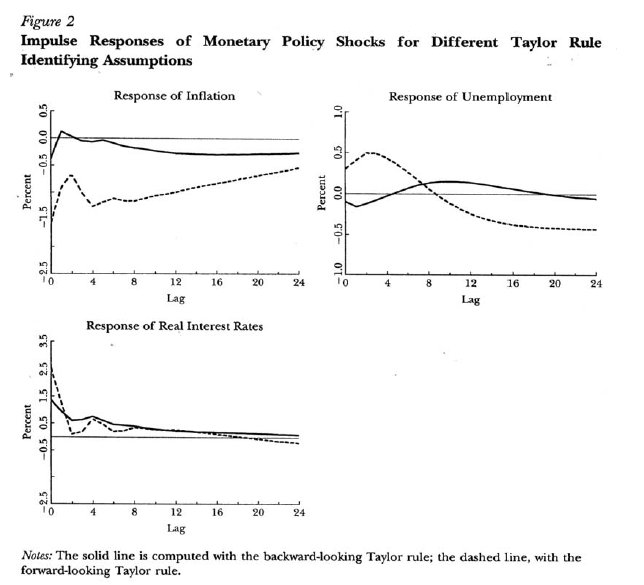
\includegraphics{/R_git/fig2_jep.png}
\end{frame}

\begin{frame}{Assessment}
\protect\hypertarget{assessment}{}
VARs are good at capturing co-movements of multiple time series.
Granger-causality tests, impulse response functions and variance
decompositions are well-accepted and widely used. Small VARs have become
the benchmarks against which new forecasting systems are judged.

Sims (1993) allows for time-varying parameters to capture important
drifts in coefficients. Adding variables involves costs. A 9-variable,
four lag VAR as 333 unknown coefficients (including intercepts).
Estimation of all of these requires restrictions. Bayesian approaches
have helped control the number of parameters in large VAR models.

Structural inference is tougher. A lot of the success of these models
depends upon evaluation of shocks. VAR shocks reflect omitted variables.
If the omitted variables (factors or information) correlate with
included variables, then the estimates will contain omitted variable
bias. Also, if agents are forward looking, impulse responses may suggest
bizarre causal responses.
\end{frame}

\begin{frame}
Changing policy rules may lead to misspecification in constant parameter
structural VARs just as they might in standard multi-equation structural
models.

Researchers also seem to be attempting to rationalize a specific causal
relationship in order to be able to justify a 7particular recursive
ordering so that their structural VAR collapses to a recursive VAR,
which makes analysis easier. With regard to forecast error variances,
Spencer (JMCB, 1989), finds: Ordering of variables: ordering of the
variables is critically important. It is of greater importance for
temporally aggregated data since the contemporaneous correlation of the
pre-orthogonalized aggregated data is likely to be greater. There is
less problem for monthly data than for quarterly, semi-annual, and
annual data.

Trend removal: the method of detrending can make a substantial
difference to variance decomposition results. Lag length: In a mrpy
model, a second year of lags to the

VAR gives increased estimates of the importance of money in explaining
industrial production. Adding lags also seems to improve the stability
of results across orderings. Level of temporal aggregation: While
aggregation may reduce noise in series, it increases cont. correlation.
\end{frame}

\end{document}
